\chapter{Experimentation}
\label{sec:Experimentation}

The intuition behind developing a CNN on this dataset is novel. Many related works demonstrate the feasibility of using CNN models to classify or segment SAR imaging \cite{SAR-U-Net}, but tend not to explore regression tasks. This could be a result of minimal data like the set derived for this study being accessible to the public. Furthermore, attempting to relate IS-2 footprints to high resolution SAR imaging involves deriving information from single-channel imagery of low pixel dimension. Compounded with the 33$\%$ yield of anticipated data from the ICEYE image, the limited data problem is exacerbated. 

\section{Setup}
The coincident data is first extracted from the ICEYE imagery, yielding 4,683 17x17 tiles with associated LiDAR measurements. The selected densities used for interpolation are as follows, where the snow density is drawn from historical measurements during the month of January \cite{warren1999snow}.

\begin{figure}[h]
  \[
  \begin{aligned}[t]
    \rho_i &=  \text{Density of sea ice }(916 \frac{kg}{m^3}) \\   %	It'd be perfect to place the diagram of the sheet in the white space generated here in latex
    \rho_s &=  \text{Density of snow }(300 \frac{kg}{m^3}) \\   %	It'd be perfect to place the diagram of the sheet in the white space generated here in latex
    \rho_w &=  \text{Density of water }(1024 \frac{kg}{m^3}) \\   %	It'd be perfect to place the diagram of the sheet in the white space generated here in latex
  \end{aligned}
\]
\end{figure}
  
Using Equation 1.1, each tile's elevation readings are converted to their associated thickness. Some values of freeboard are negative, so they are interpreted to represent the absence of snow and an overestimate of sea ice surface elevation. The negative freeboard values are then added to the sea ice surface elevation to compensate. Each tile's interpolated ice thickness can be visualized in Figure 3.1.

\begin{figure}[h!]
	\centering
	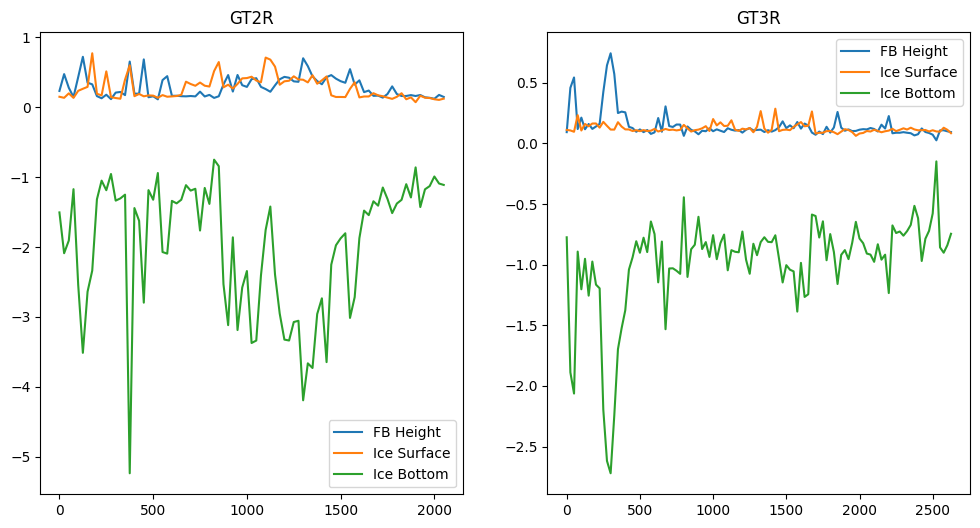
\includegraphics[width=\textwidth]{../research-resources/ice-sat-2/coincident-ice-profile.png}
	\caption{Interpolated Ice Thickness}
	\label{fig:ice-thickness-interpolation}
\end{figure}

The experimental model for the data is a feed forward neural network, consisting of 3 convolutional layers and 3 fully connected layers. Each convolutional layer is followed by the ReLU activation function, and the model uses the ADAM optimizer at a $10^{-5}$ learning rate based upon the L1 loss function. Given the already minimal pixel-space dimension, pooling and filter dilation are avoided to better preserve information across layers of the network.

The intuition behind experimenting with a simple model is rooted largely from the sparseness of existing studies attempting regression on low-resolution single channel images. Studies on classification, however, find that wider datasets (data that spans more classes) benefit from a larger amount of neurons in fully connected layers \cite{BASHA2020112}. Regression tasks for continuous numbers can be thought of as infinite classification, thus supporting the decision to implement multiple fully connected layers of large dimension. Some classification studies find value in decreasing filter sizes with model depth \cite{ganj2023lrnet}, but for this model, kernel size is decreased from 5 to 3 only between the first and second convolution layer.

\begin{figure}
  \centering
  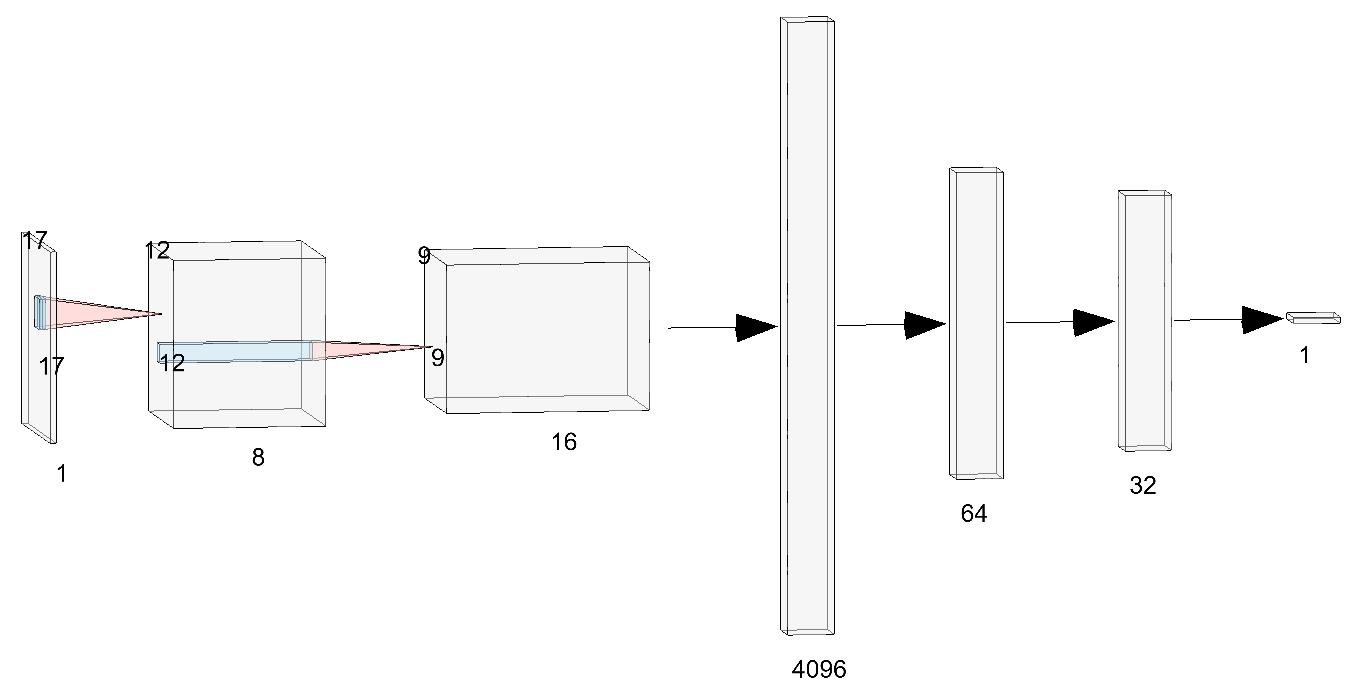
\includegraphics[width=0.8\textwidth]{../research-resources/CNN/model-architecture.png}
	\caption{CNN Architecture}
	\label{fig:cnn-model}
\end{figure}

The training process for the model uses 80\% of the data to train and 20\% to test, a batch size of 32 to promote faster convergence, random flipping and rotation to prevent over-fitting, and scaling of each pixel to the [0,255] color range. The model is trained over 100 epochs.


\section{Model Results}

\begin{figure}[hbt!]
	\centering
  \subfigure[]{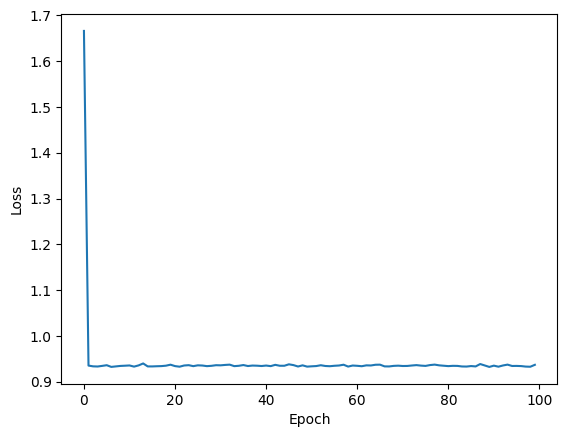
\includegraphics[width=.48\linewidth]{../research-resources/CNN/no-convergence.png}}
  \subfigure[]{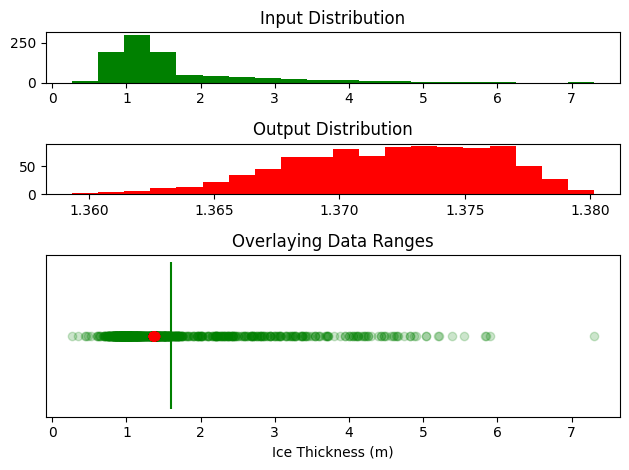
\includegraphics[width=.48\linewidth]{../research-resources/CNN/unconverged-distribution.png}}
	\caption[Model Performance]{(a) Model Convergence (b) Model Predictions}
	\label{fig:model-results}
\end{figure}

After 100 epochs, the model fails to converge (Figure 3.3). The L1 Loss function plateaus at $\approx0.66$, and the model predicts a concentrated set of values slightly lower than the test set's mean. This value can be explained by the L1 Loss function's insensitivity towards outliers, as the mean (vertical bar) would be shifted right because of the skew in the input distribution.

The model reports an R2 value of -.056 and an RMSE of 0.9996, both of which suggest the model does not fit the data at all. The normalized RMSE is 0.14, which seemingly better, is only the result of the relatively narrow range of ice thicknesses being predicted in the testing set. Minor changes to the activation function and hyper-parameters yielded no significant difference to the model's evaluation metrics, nor did they assist in loss convergence. The inadequacies demonstrated by these tests suggest a more sophisticated architecture would be needed to better associate these low-resolution 1 channel images with their interpolated thickness measurements.

% \section {U-Net}